\section{Database and selection of test subjects}
As test sample a data set of XXX\todo{how many?} ICAO compliant pictures were given. In order to get promising morph results, a subset of XX \todo{number} pairs of photos were selected for manual morphing \ref{manual_morph} where as the automatic morphing algorithm \ref{automatic_morph} was applied on all data sets. For manual  morphing only pairs with a visually high coincidence are considered because the aceptance rate of the comparison algorithem is expected to be higher. 
In summation XX manual and XXX automatic morphs are issued in this paper. 


\section{Morphing of Faces}
The main task during the morphing of two pictures is to detect characteristics and place landmarks as an advince for the algorithm. This can be done completely automatic or with support of an user. In this paper both way are discussed.  
\subsection{Automatic morphing}
\label{automatic_morph}
\subsubsection{Results}

\subsection*{Manual morphing}
\label{manual_morph}
In contrast to the automatic face morphing approach, manual morphing is discussed in this section. 

To achieve morphes, the open source software GNU Image Manipulation Software (GIMP) (Version 2.8.16) with the GIMP Animation Package (GAP) (Version 2.6) was selected for this paper. Morphing with GAP follows the simple approach of manually placing connected landmarks at characterizing points in both faces. The algorithm shifts the landmarks from face one to face two. In addition to this the color of the skin is transmitted. 

%\subsubsection*{Morphing setup}
For the test samples 100 - 125 landmarks were placed, depending on the face characteristics. The output contains a sequence of 30 photos which show different stages of the morphing procedure. 
In figure \ref{fig1} a two subjects and three morphing stages (5, 15 and 25) are shown. The visual inspection of \ref{1c} shows biometric features of both subjects whereas \ref{1b} and \ref{1d} has more similarity to the closer subject but also covers features of the other subject.
A manual post production of the morphs is not necessary because potential revealing details, like the interference \todo{?} of the clothes, glasses or hair is not considered as characteri


\cite{vukadinovic2005fully}
\begin{figure} 
	\centering
	\subfloat[Subject 1]{%
		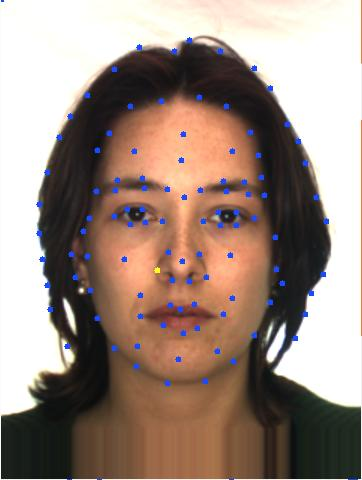
\includegraphics[width=0.45\linewidth]{Resources/manualmorph01.jpg}}
	\label{1a}\hfill
	\subfloat[Morph no. 5]{%
		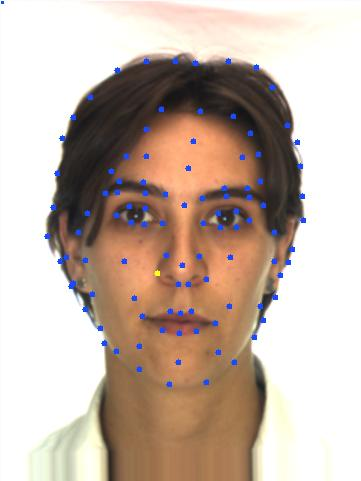
\includegraphics[width=0.45\linewidth]{Resources/manualmorph02.jpg}}
	\label{1b}\\

	\caption{Example of two ICAO compliant photos (1a and 1e) and morphs at stage 5 (1b), 15 (1c) and 25 (1d)}
	\label{fig1} 
\end{figure}

\subsubsection*{Results}
\todo{compare to automatic results when there.}
\begin{figure} 
	\centering
	\subfloat[Subject 1]{%
		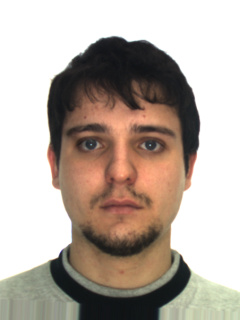
\includegraphics[width=0.45\linewidth]{Resources/p1.jpg}}
	\label{1a}\hfill
	\subfloat[Morph no. 5]{%
		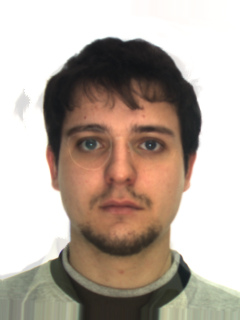
\includegraphics[width=0.45\linewidth]{Resources/m1.jpg}}
	\label{1b}\\
	\subfloat[Morph no. 15]{%
		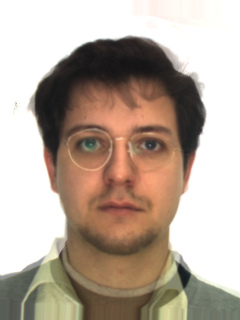
\includegraphics[width=0.45\linewidth]{Resources/m2.jpg}}
	\label{1c}\hfill
	\subfloat[Morph no. 25]{%
		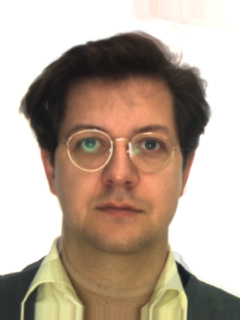
\includegraphics[width=0.45\linewidth]{Resources/m3.jpg}}
	\label{1d}\hfill
	\subfloat[Subject 2]{%
		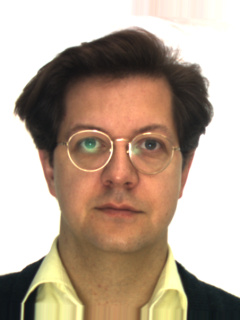
\includegraphics[width=0.45\linewidth]{Resources/p2.jpg}}
	\label{1e} 
	\caption{Example of two ICAO compliant photos (1a and 1e) and morphs at stage 5 (1b), 15 (1c) and 25 (1d)}
	\label{fig1} 
\end{figure}

\todo[inline]{Detailed description of the morphs}